\chapter{Evaluation}
%klare begründung => Anforderung erfüllt ja oder nein


\section{RANSAC Algorithm}

\subsection{Tests on singular synthetic cube}

A unit cube will be used as a test object to evaluate the RANSAC algorithm.
The cube has been generated with a side length of 1 and a sampling rate of 0.01.
This would equate to a cube with a side length of 1m and a distance of 1cm between points in the real world,
which is comparable to what is provided by the Raw Depth API\@.

\subsubsection{Resilience to Noise}
In figure~\ref{fig:test-synthetic-data}, the unit cube is shown with varying noise levels.


\begin{figure}[ht!]
    \centering
    % First row
    \begin{subfigure}[b]{0.25\textwidth}
        \centering
        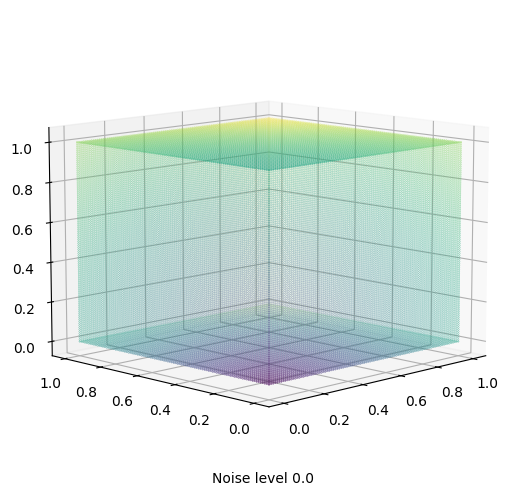
\includegraphics[width=0.9\linewidth]{python/plots/cube_points/data/cube_points_00}
    \end{subfigure}%
    \begin{subfigure}[b]{0.25\textwidth}
        \centering
        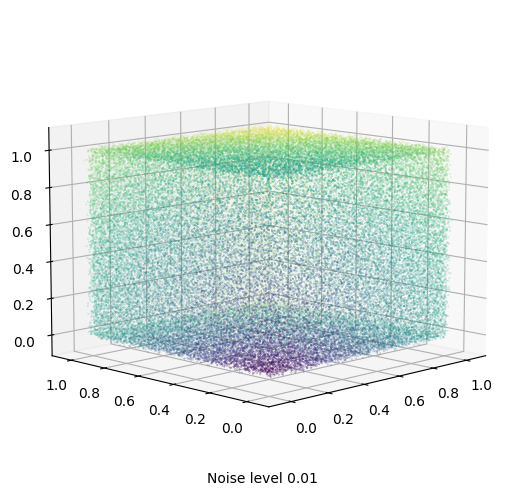
\includegraphics[width=0.9\linewidth]{python/plots/cube_points/data/cube_points_01}
    \end{subfigure}%
    \begin{subfigure}[b]{0.25\textwidth}
        \centering
        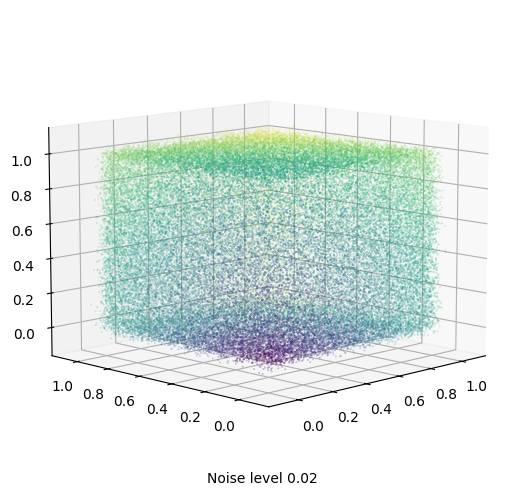
\includegraphics[width=0.9\linewidth]{python/plots/cube_points/data/cube_points_02}
    \end{subfigure}%
    \begin{subfigure}[b]{0.25\textwidth}
        \centering
        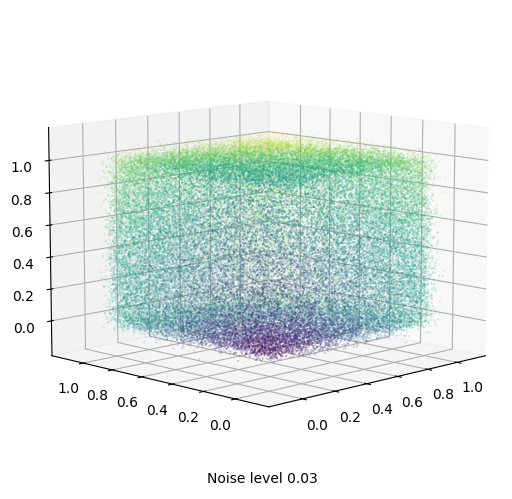
\includegraphics[width=0.9\linewidth]{python/plots/cube_points/data/cube_points_03}
    \end{subfigure}%

%    \vspace{0.5em}

    \begin{subfigure}[b]{0.25\textwidth}
        \centering
        
\includegraphics[width=0.9\linewidth]{python/plots/cube_points/data/cube_primitives_00}
        \caption{Noise level 0.00}
    \end{subfigure}%
    \begin{subfigure}[b]{0.25\textwidth}
        \centering
        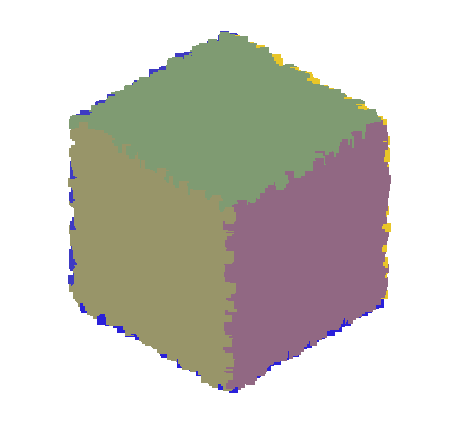
\includegraphics[width=0.9\linewidth]{python/plots/cube_points/data/cube_primitives_01}
        \caption{Noise level 0.01}
    \end{subfigure}%
    \begin{subfigure}[b]{0.25\textwidth}
        \centering
        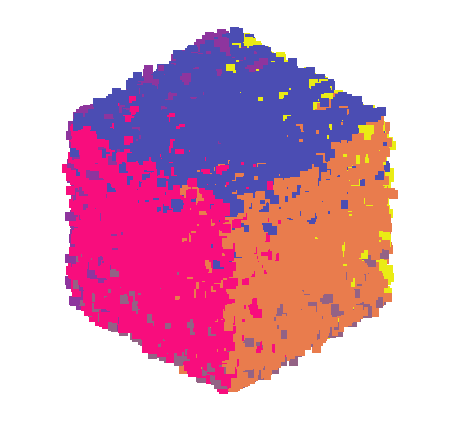
\includegraphics[width=0.9\linewidth]{python/plots/cube_points/data/cube_primitives_02}
        \caption{Noise level 0.02}
    \end{subfigure}%
    \begin{subfigure}[b]{0.25\textwidth}
        \centering
        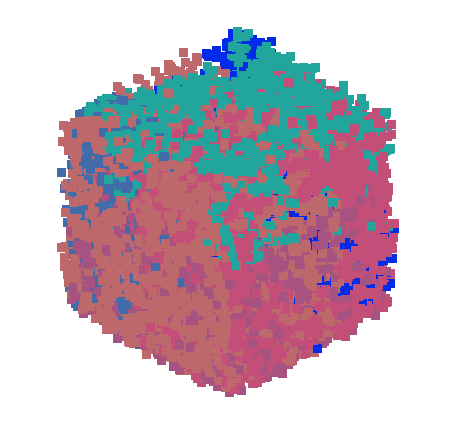
\includegraphics[width=0.9\linewidth]{python/plots/cube_points/data/cube_primitives_03}
        \caption{Noise level 0.03}
    \end{subfigure}%

    \caption{Unit cube with varying noise level}
    \label{fig:test-synthetic-data}
\end{figure}

\subsubsection{Resilience to missing Data}

As a big problem of depth from motion techniques is the lack of depth information in areas with minimal texture,
the resilience to missing data is crucial.
In the following data, points towards the center of the cubes surfaces have been removed.
This mimics the structure of the data of real world data from the Depth API,
as edges are often detected more accurately than surfaces.
